\documentclass{../../presentation}

\title{PSE - Vorkurs}
\author{Tobias, Philipp, Linus, Tillmann}
\institute{FIUS - Fachgruppe Informatik Universität Stuttgart}
\date{\today}

\makeatletter
\renewcommand{\lecture@pathprefix}[1]{../../logos/}
\makeatother

\usepackage{todonotes}
\setuptodonotes{inline}

\begin{document}

\begin{frame}
  \titlepage
\end{frame}

\begin{frame}
  \listoftodos
\end{frame}

\section{Introduction}

\begin{frame}[fragile]
  \frametitle{WLAN}
  Die Universität bietet ein Gast WLAN an jedoch wollen wir in das offizielle WLAN der Universität einsteigen.
  \newline
  \begin{itemize}
    \item iOS und Android
    \item Windows
    \item MacOS
    \item Linux
  \end{itemize}
\end{frame}

\begin{frame}[fragile]
  \frametitle{WLAN - iOS und Android}
  \begin{itemize}
    \item Im AppStore bzw. Playstore nach \enquote{geteduroam} suchen und die App installieren
    \item Dann nach Universität Stuttgart suchen 
    \item Nun Student wählen und eure Daten eingeben
    \item \texttt{stxxxxxx@stud.uni-stuttgart.de} - Benutzername
    \item Und eurer Passwort eingeben
    \item Nun auf Verbinden klicken und fertig
  \end{itemize}
\end{frame}

\begin{frame}[fragile]
  \frametitle{WLAN - Windows}
  \begin{itemize}
    \item Im Internet auf \href{https://geteduroam.app}{\enquote{geteduroam.app}} gehen und die Windows Version herunterladen 
    \item Dann nach Universität Stuttgart suchen 
    \item Nun Student wählen und eure Daten eingeben
    \item Nun auf Verbinden klicken und fertig
  \end{itemize}
\end{frame}

\begin{frame}[fragile]
  \frametitle{WLAN - MacOS}
  \begin{itemize}
    \item Im Internet auf \href{http://uni-stuttgart.de/eduroam}{\enquote{uni-stuttgart.de/eduroam}} gehen
    \item und als Gruppe \enquote{Student} wählen
    \item Lädet das Konfigurationspaket herunter
    \item In euren Systemeinstellungen auf \enquote{Geräteverwaltung} gehen
    \item Nun über das Plus-Symbol das Konfigurationspaket hinzufügen
    \item \texttt{stxxxxx} - Benutzername 
    \item Und euer Passwort eingeben
    \item Nun auf Verbinden klicken und fertig
  \end{itemize}
\end{frame}

\begin{frame}[fragile]
  \frametitle{WLAN - Linux}
  \begin{itemize}
    \item Im Internet auf \href{http://uni-stuttgart.de/eduroam}{\enquote{uni-stuttgart.de/eduroam}} gehen
    \item Als Benutzergruppe \enquote{Student} wählen
    \item Unten links auf \enquote{einen anderen Installer auswählen} klicken
    \item \enquote{Linux} auswählen
    \item Über den Button das Pythonskript herunterladen
    \item Im Terminal mit \texttt{\$ python3 [Dateipfad zum Pythonskript]} ausführen
    \item Den Anweisungen folgen und Benutzername (\texttt{stxxxxxx@stud.uni-stuttgart.de}) sowie Passwort eingeben
  \end{itemize}
\end{frame}

\begin{frame}
  \frametitle{IntelliJ IDEA}
  \textbf{\achtung{} Wir werden uns Lediglich auf IntelliJ IDEA konzentrieren, wenn ihr eine andere IDE nutzen wollt, können wir keinen Support garantieren. }
  \newline  
  \begin{itemize}
    \item Wir laden uns erst die JetBrains Toolbox herunter, um die IDE zu installieren
    \item Dann installieren wir IntelliJ IDEA Community Edition
  \end{itemize}
\end{frame}

\begin{frame}
   
\includegraphics[width=1\linewidth]{img/memeIDE.jpg}
\end{frame}

\begin{frame}
  \frametitle{IntelliJ IDEA - Installation}
  \begin{tikzpicture}[remember picture,overlay]
    \node[at=(current page.center), anchor=center, yshift=-2] {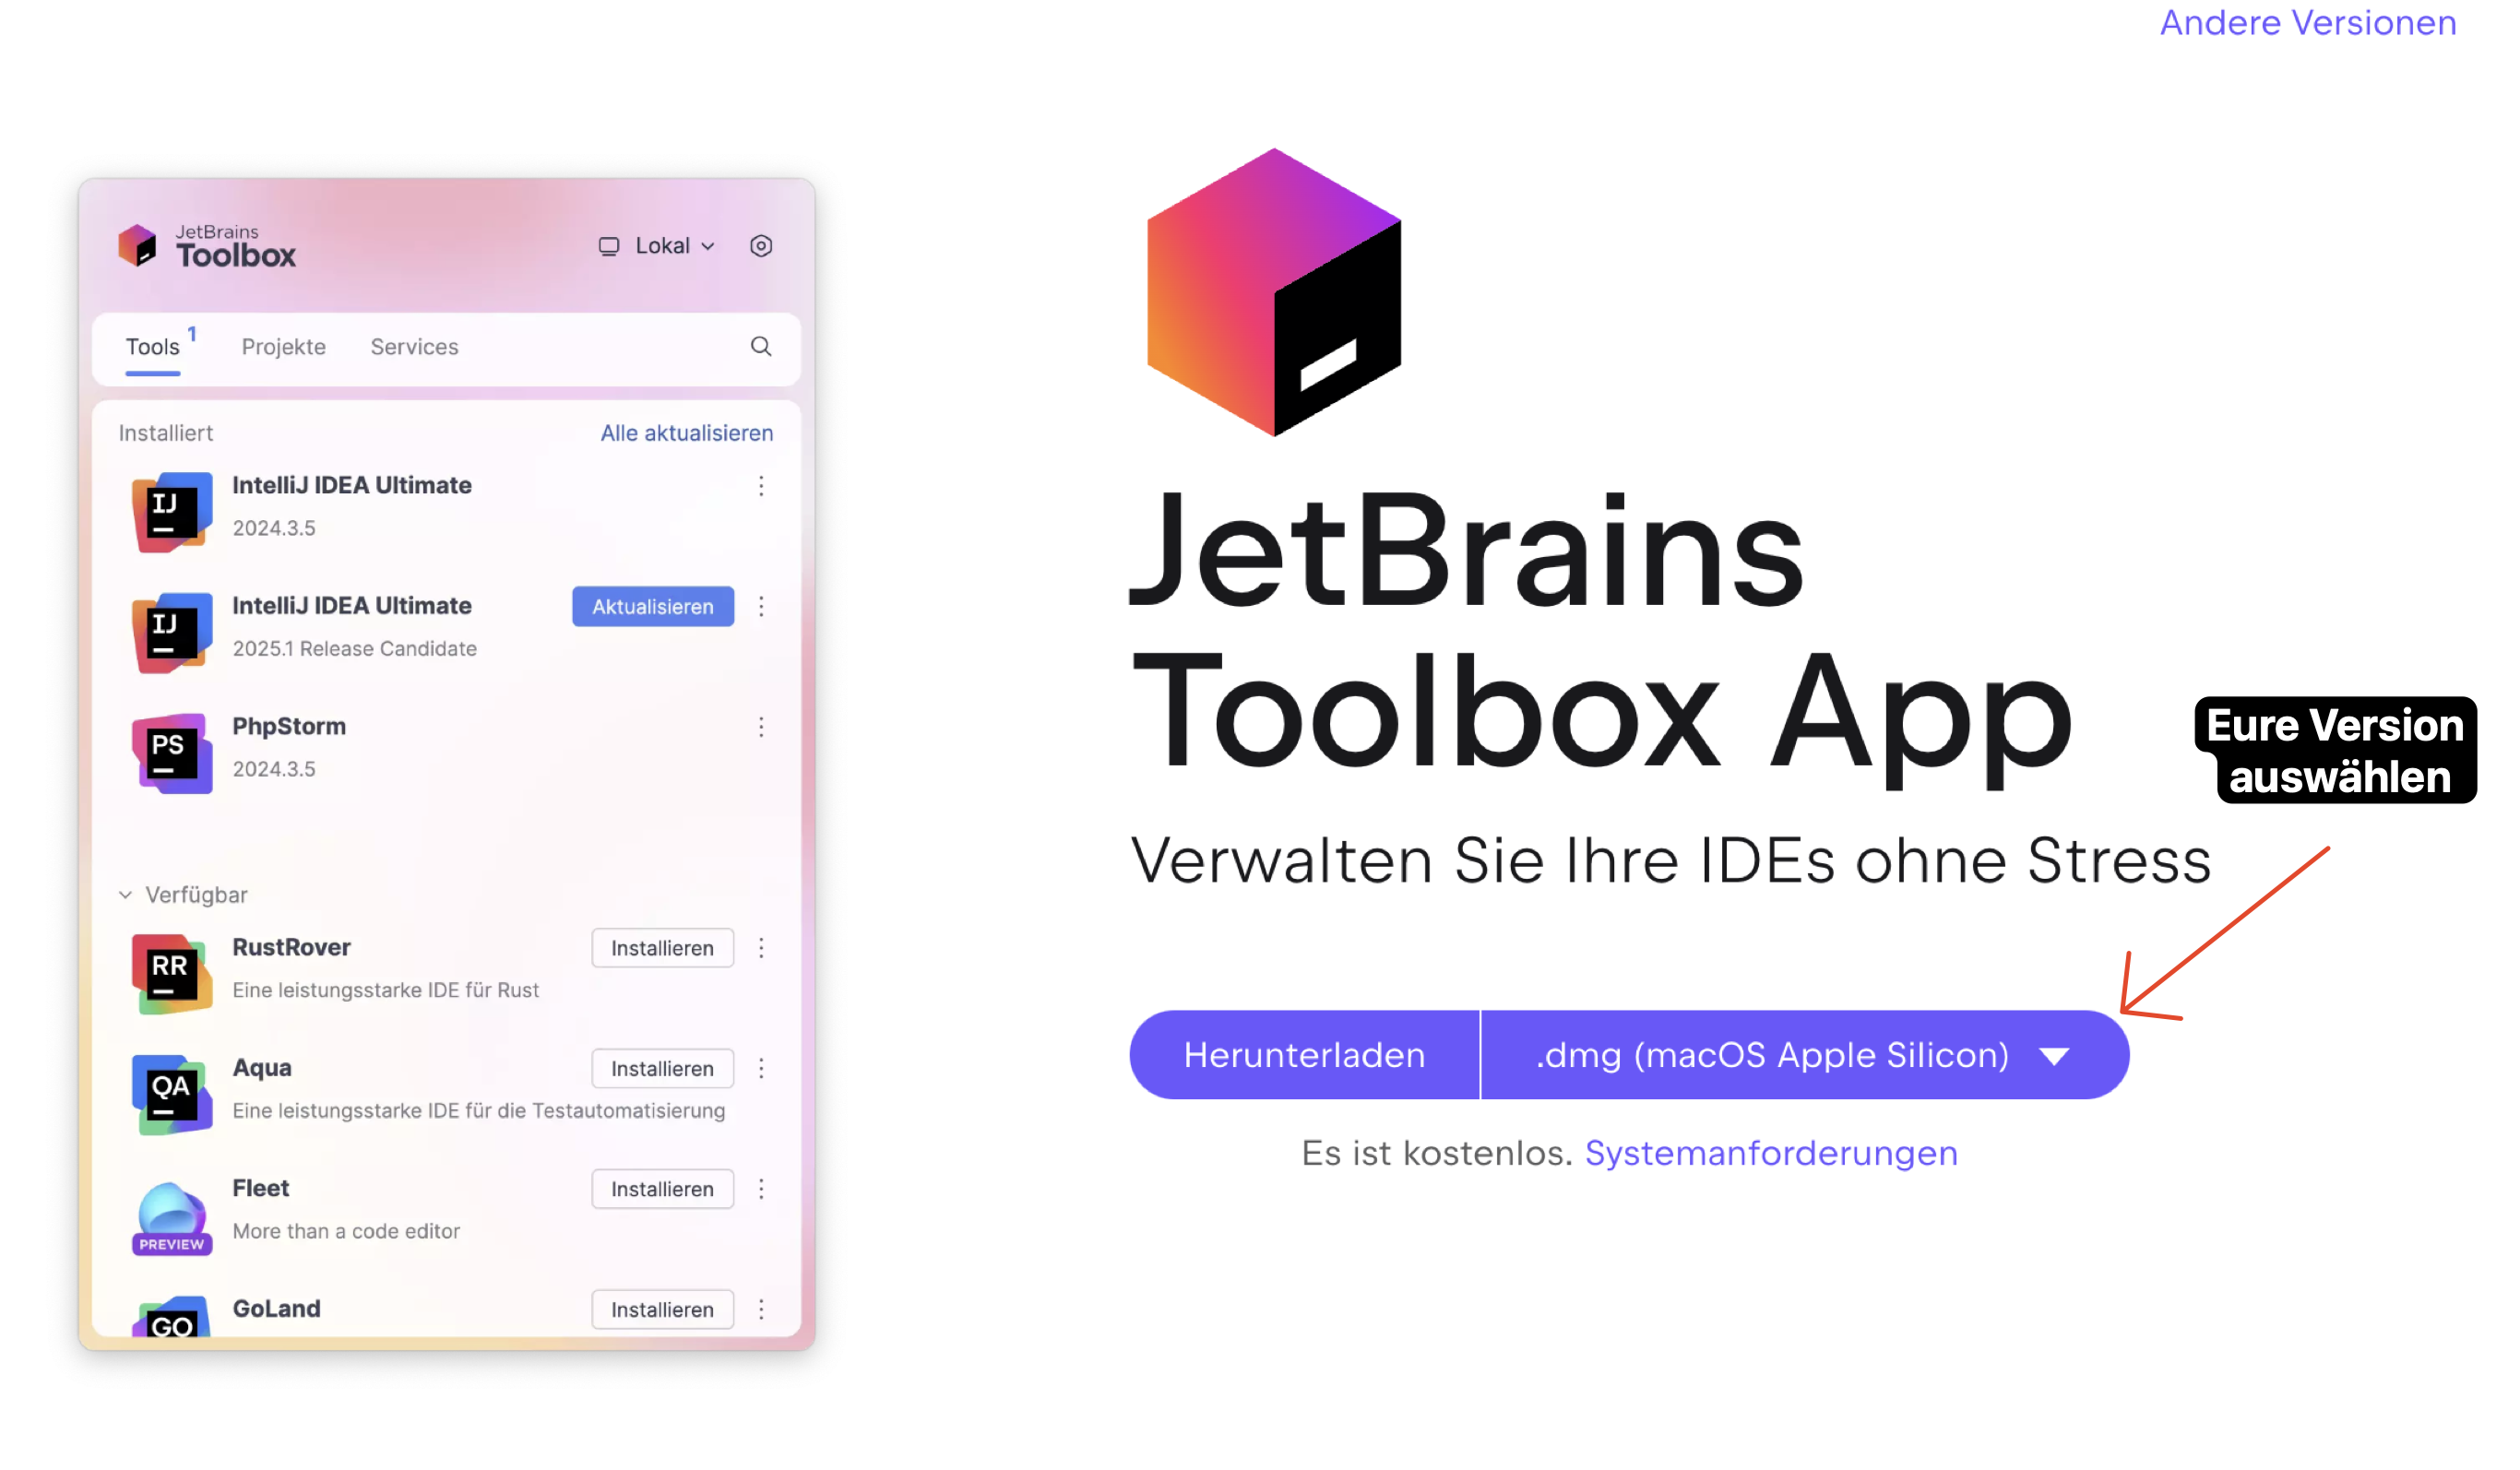
\includegraphics[width=1\linewidth]{img/toolBoxDownload.png}};
    \node[at=(current page.north), anchor=north, align=center, yshift=-1.2cm] {Geht auf \href{https://www.jetbrains.com/de-de/toolbox-app/}{\texttt{\enquote{jetbrains.com/toolbox-app/}}} und ladet die Toolbox herunter.};
  \end{tikzpicture}
\end{frame}

\begin{frame}
  \frametitle{IntelliJ IDEA - Installation}
  \begin{tikzpicture}[remember picture,overlay]
    \node[at=(current page.east), anchor=east, yshift=-2] {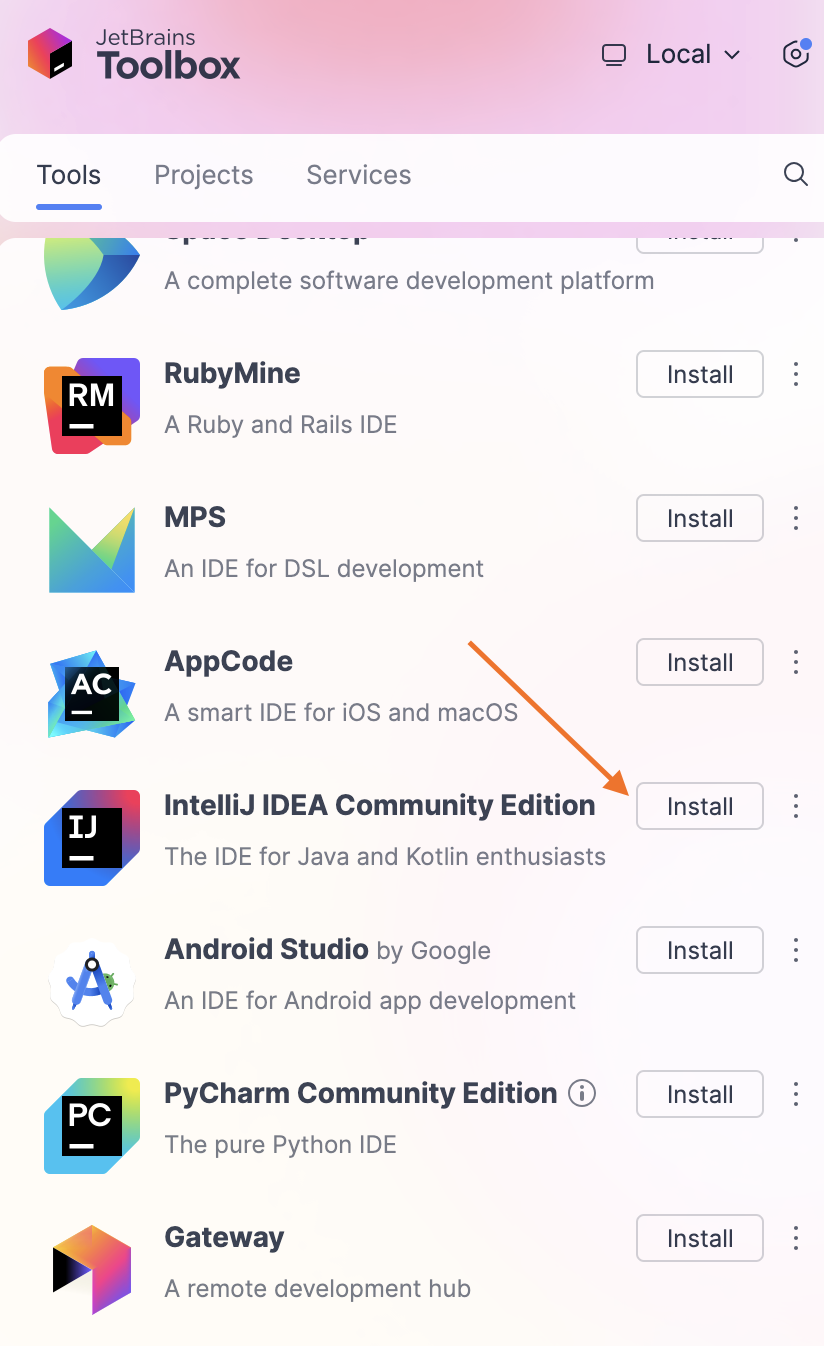
\includegraphics[width=.35\linewidth]{img/IntelliJDownload.png}};
    \node[at=(current page.west), anchor=west, align=center, yshift=0cm, xshift=2cm, text width=8cm] {Nach der Installation der Toolbox öffnet sich ein Fenster, in dem ihr die IDE auswählen könnt, die ihr installieren wollt. Wählt \enquote{IntelliJ IDEA Community Edition} aus und klickt auf \enquote{Install}. \newline \todo{Besser machen}};
  \end{tikzpicture}
\end{frame}

\begin{frame}
  \frametitle{JDK - Installation}
  Wir benötigen ein JDK (Java Development Kit), um Java Programme zu schreiben und auszuführen.
  \newline
  \begin{itemize}
    \item \achtung{} MacOS: auf File/ Datei gehen oben links in der Menüleiste
    \item Nun auf \texttt{Project Structure} klicken
    \item Dann auf \texttt{SDKs} klicken
    \item Dann auf das Plus-Symbol klicken und auf \texttt{Download JDK} klicken
  \end{itemize}
\end{frame}



\end{document}
